\let\lesson\undefined
\newcommand{\lesson}{\phantomlesson{Bài 10: Lực từ - Cảm ứng từ}}
\chapter[Cảm ứng từ gây ra bởi dòng điện trong dây dẫn có hình dạng đặc biệt (Đọc thêm)]{Cảm ứng từ gây ra bởi dòng điện trong dây dẫn có hình dạng đặc biệt (Đọc thêm)}
\section{Lý thuyết}
\subsection{Cảm ứng từ gây ra bởi dòng điện trong dây dẫn có hình dạng đặc biệt đặt trong không khí}
\subsubsection{Từ trường của dòng điện chạy trong dây dẫn thẳng, dài}
\begin{center}
	\begin{tikzpicture}
		\coordinate (O) at (0,0);
		\coordinate (M) at ($(O)+(-15:1.9)$);
		\coordinate (N) at ($(M)+(45:1.5)$);
		\node[draw, line width=1pt, fill=white, trapezium ,minimum width=8cm, trapezium left angle=60, trapezium right angle=120, anchor=center] at (O) {};
		\node[draw,blue, line width=1pt, fill=white, ellipse, minimum width=4cm, minimum height=2.5cm, anchor=center,
		decoration={markings, mark=at position 0.125 with {\arrow{stealth}}},
		decoration={markings, mark=at position 0.625 with {\arrow{stealth}}},
		postaction={decorate}
		] at (O) {};
		\tkzMarkRightAngle[draw=black,size=0.2](O,M,N);
		\draw[green!60!black, line width=1.5pt, decoration={markings, mark=at position 0.75 with {\arrow{stealth}}},
		postaction={decorate}] (O)--($(O)+(0,3)$);
		\draw[line width=1pt,dashed] (O)--(M);
		\draw[line width=1.5pt,green!60!black, dashed] (O)--($(O)-(0,1.5)$);
		\draw[green!60!black, line width=1.5pt] ($(O)-(0,1.5)$)--($(O)-(0,3)$);
		\draw[red, line width=1.5pt, -latex] (M)--($(M)+(45:1.5)$);
		\filldraw[black] (M) circle (2pt) node[below right] {M};
		\node[green!60!black, above right] at (0,2.25) {$I$};
		\node[red, above left] at (N) {$\vec{B}$};
		\node[above]  at ($(O)!0.5!(M)$) {$r$};
		
	\end{tikzpicture}
\end{center}
Độ lớn cảm ứng từ tại một điểm cách dòng điện thẳng dài vô hạn một đoạn $r$:
\begin{equation}
	B=2\cdot10^{-7}\dfrac{I}{r}
\end{equation}
\subsubsection{Từ trường của dòng điện chạy trong dây dẫn tròn}
\begin{center}
	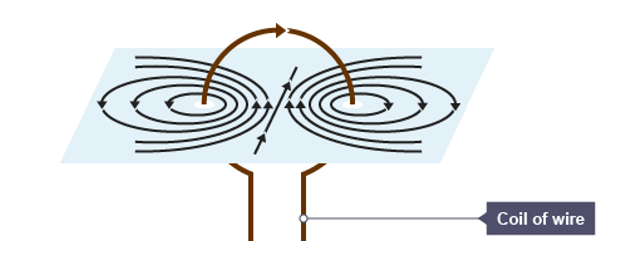
\includegraphics[width=0.4\linewidth]{../figs/VN12-Y24-PH-SYL-019-1}
\end{center}
Độ lớn cảm ứng từ tại tâm dòng điện tròn có $N$ vòng dây và có bán kính $R$:
\begin{equation}
	B=2\pi\cdot10^{-7}\dfrac{NI}{R}
\end{equation}
\subsubsection{Từ trường của ống dây có dòng diện chạy qua}
\begin{center}
	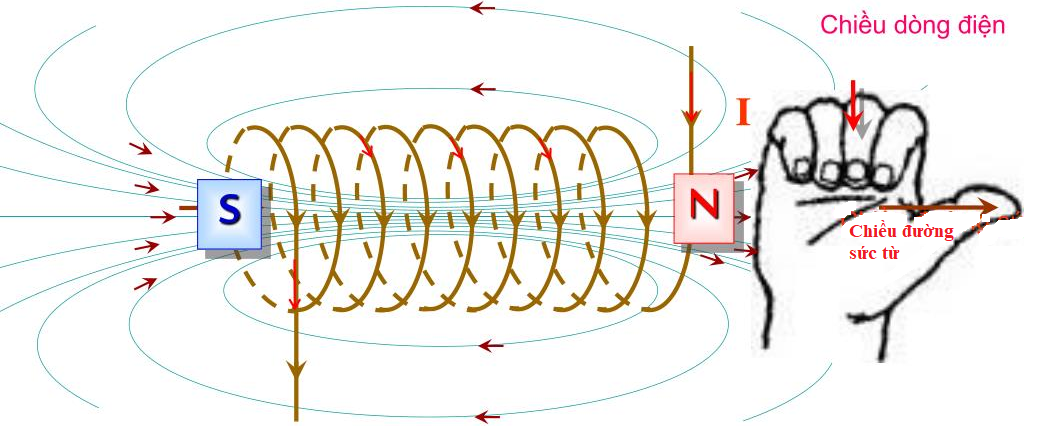
\includegraphics[width=0.6\linewidth]{../figs/VN12-Y24-PH-SYL-019-2}
\end{center}
Độ lớn cảm ứng từ bên trong ống dây có chiều dài $L$ và $N$ vòng dây (chiều dài ống dây rất lớn so với bán kính vòng dây):
\begin{equation}
	B=4\pi \cdot10^{-7}\dfrac{NI}{L}
\end{equation}
với $I$ là cường độ dòng điện trong dây dẫn.
\subsection{Nguyên lý chồng chất từ trường}
Xét hệ có $n$ dây dẫn lần lượt mang các dòng điện có cường độ dòng điện là $I_1$, $I_2$, \dots, $I_n$. Cảm ứng từ do mỗi dòng điện gây ra tại điểm M trong không gian là $\vec{B}_1$, $\vec{B}_2$,\dots,$\vec{B}_n$. Khi đó cảm ứng từ tổng hợp tại điểm M là:
\begin{equation}
	\vec{B}_\text{M}=\vec{B}_1+\vec{B}_2+\dots+\vec{B}_n
\end{equation}
\section{Mục tiêu bài học - Ví dụ minh hoạ}
\begin{dang}{Xác định được độ lớn cảm ứng từ do dòng điện trong dây dẫn có hình dạng đặc biệt gây ra}
	\viduii{2}
{Một dòng điện $\SI{20}{\ampere}$ chạy trong một dây dẫn thẳng, dài vô hạn, đặt trong không khí. Xác định độ lớn cảm ứng từ do dòng điện trong dây gây ra tại điểm cách dây $\SI{10}{\centi\meter}$.

}
{\hide{
Cảm ứng từ do dòng điện trong dây dẫn gây ra tại điểm cách dây đoạn $r=\SI{10}{\centi\meter}$:
$$B=2\cdot10^{-7}\dfrac{I}{r}=	2\cdot10^{-7}\cdot\dfrac{\left(\SI{20}{\ampere}\right)}{\left(\SI{0.1}{\meter}\right)}=\SI{4E-5}{\tesla}.$$

}

}

\viduii{2}
{Một vòng dây tròn bán kính $\SI{30}{\centi\meter}$ có dòng điện chạy qua. Cảm ứng từ do dòng điện gây ra tại tâm vòng dây có độ lớn $\SI{3.14E-5}{\tesla}$. Cường độ dòng điện chạy trong vòng dây là bao nhiêu?

}
{\hide{
Cảm ứng từ do dòng điện trong dây dẫn tròn gây ra tại tâm vòng dây:
$$B=2\pi\cdot10^{-7}\dfrac{I}{R}.$$
Cường độ dòng điện chạy trong vòng dây:
$$I=\dfrac{BR}{2\pi\cdot10^{-7}}=\dfrac{\left(\SI{3.14E-5}{\tesla}\right)\cdot\left(\SI{0.3}{\meter}\right)}{2\pi\cdot10^{-7}}=\SI{15}{\ampere}.$$
}

}
	
	\viduii{3}
	{Dùng một dây đồng có phủ một lớp sơn cách điện mỏng, quấn quanh một hình trụ dài $L=\SI{50}{\centi\meter}$, có đường kính $d=\SI{4}{\centi\meter}$ để làm một ống dây. Sợi dây quấn ống dây có chiều dài $\ell=\SI{314}{\centi\meter}$ và các vòng dây được quấn sát nhau. Hỏi nếu cho dòng điện cường độ $I=\SI{0.4}{\ampere}$ chạy qua ống dây, thì độ lớn cảm ứng từ bên trong ống dây bằng bao nhiêu?
	
}
{\hide{
Số vòng dây quấn trên ống dây:
$$N=\dfrac{\ell}{\pi d}.$$
Cảm ứng từ bên trong ống dây:
$$B=4\pi\cdot10^{-7}\dfrac{NI}{L}=4\cdot10^{-7}\dfrac{\ell I}{ Ld}=4\cdot10^{-7}\dfrac{\left(\SI{3.14}{\meter}\right)\cdot\left(\SI{0.4}{\ampere}\right)}{\left(\SI{4E-2}{\meter}\right)\cdot\left(\SI{0.5}{\meter}\right)}=\SI{2.512E-5}{\tesla}.$$	

}

}
\end{dang}
\begin{dang}{Xác định được cảm ứng từ tổng hợp}
	\viduii{3}
	{Hai dây dẫn thẳng, rất dài, đặt song song, cách nhau $\SI{10}{\centi\meter}$ trong không khí, có hai dòng điện ngược chiều, có cường độ $I_1=\SI{6}{\ampere}$; $I_2=\SI{12}{\ampere}$ chạy qua. Xác định cảm ứng từ tổng hợp do hai dòng điện này gây ra tại điểm M cách dây dẫn mang dòng $I_1$ đoạn $\SI{5}{\centi\meter}$ và cách dây dẫn mang dòng $I_2$ đoạn $\SI{15}{\centi\meter}$.
	
}
{\hide{
\begin{center}
	\begin{tikzpicture}
		\coordinate (A) at (0,0);
		\coordinate (B) at (10,0);
		\coordinate (M) at (-5,0);
		
	
		\draw[red, line width=1.5pt, -stealth] (M)--($(M)+(0,-3)$);
		\draw[green!60!black, line width=1.5pt, -stealth] (M)--($(M)+(0,2)$);
		\draw[blue, line width=1.5pt, -stealth] (M)--($(M)+(0,-1)$);
		\draw[line width=1pt, dashed] (M)--(B);
		\node[circle, red, fill=white, inner sep=0pt, minimum size=0pt] at (A) {\LARGE$\odot$};
		\node[below] at ($(A)+(0,-.25)$)  {A};
		\node[below] at ($(B)+(0,-.25)$)  {B};
		\node[above] at ($(A)+(0,0.25)$)  {$I_1$};
		\node[above] at ($(B)+(0,.25)$)  {$I_2$};
		\node[red, left] at ($(M)-(0,3)$) {$\vec{B}_{1M}$};
		\node[green!60!black, left] at ($(M)+(0,2)$) {$\vec{B}_{2M}$};
		\node[blue, left] at ($(M)+(0,-1)$) {$\vec{B}_M$};
		\node[circle, green!60!black, fill=white, inner sep=0pt, minimum size=0pt] at (B) {\LARGE$\otimes$};
			\filldraw[black] (M) circle (2pt) node[left] {M};
	\end{tikzpicture}
\end{center}	
Từ trường do các dây dẫn gây ra tại M:
\begin{align*}
	\begin{cases}
		B_{1M}=\SI{2E-7}{}\dfrac{I_1}{\text{AM}}=\SI{2E-7}{}\dfrac{\left(\SI{6}{\ampere}\right)}{\SI{5E-2}{\meter}}=\SI{2.4E-5}{\tesla}\\
		\ \\
		B_{2M}=\SI{2E-7}{}\dfrac{I_2}{\text{BM}}=\SI{2E-7}{}\dfrac{\left(\SI{12}{\ampere}\right)}{\SI{15E-2}{\meter}}=\SI{1.6E-5}{\tesla}
	\end{cases}
\end{align*}
Vì $\vec{B}_{1M}\uparrow\downarrow\vec{B}_{2M}$ nên:
$$B_M=\left|B_{1M}-B_{2M}\right|=\SI{0.8E-5}{\tesla}.$$
}

}

\viduii{3}
{Hai dây dẫn thẳng, rất dài, đặt song song, cách nhau $\SI{15}{\centi\meter}$ trong không khí, có hai dòng điện cùng chiều, cùng cường độ $I_1=\SI{10}{\ampere}$, $I_2=\SI{5}{\ampere}$ chạy qua. Xác định điểm M mà tại đó cảm ứng từ tổng hợp do hai dòng điện này gây ra bằng 0.

}
{\hide{
		Để từ trường tổng hợp tại M bằng 0 thì:
		$$\vec{B}_M=\vec{B}_{1M}+\vec{B}_{2M}=\vec{0}\Rightarrow \vec{B}_{1M}=-\vec{B}_{2M}.$$	
	\begin{center}
		\begin{tikzpicture}
			\coordinate (A) at (0,0);
			\coordinate (B) at (15,0);
			\coordinate (M) at (10,0);
			
			\draw[line width=1pt, dashed] (A)--(B);
			\draw[red, line width=1.5pt,-stealth] (M)--($(M)+(0,2)$);
			
			\draw[green!60!black, line width=1.5pt,-stealth] (M)--($(M)-(0,2)$);
			\node[circle, green!60!black, fill=white, inner sep=0pt, minimum size=0pt] at (A) {\LARGE$\otimes$};
			\node[circle, red, fill=white, inner sep=0pt, minimum size=0pt] at (B) {\LARGE$\otimes$};
			\node[below] at ($(A)-(0,0.25)$) {A};
			\node[below] at ($(B)-(0,0.25)$) {B};
			\node[above] at ($(A)+(0,0.25)$) {$I_1$};
			\node[above] at ($(B)+(0,0.25)$) {$I_2$};
			\node[left, red] at ($(M)+(0,2)$) {$\vec{B}_{2M}$};
			\node[left, green!60!black] at ($(M)-(0,2)$) {$\vec{B}_{1M}$};
			\filldraw[black] (M) circle(2pt) node[above left] {M};
			
		\end{tikzpicture}
	\end{center}
Do hai dòng điện cùng chiều nên điểm M phải nằm trong khoảng AB:
\begin{eqnarray*}
	&&B_{1M}=B_{2M}\\
	&\Rightarrow& \dfrac{I_1}{\text{AM}}=\dfrac{I_2}{\text{BM}}\\
	&\Rightarrow& \text{AM}=2\text{BM}.
\end{eqnarray*}
Mà $\text{AM}+\text{BM}=\text{AB}=\SI{15}{\centi\meter}$ nên:
\begin{align*}
	\begin{cases}
		\text{AM}=\SI{10}{\centi\meter}\\
		\text{BM}=\SI{5}{\centi\meter}
	\end{cases}
\end{align*}
}

}
	\viduii{3}
	{Hai dây dẫn thẳng, rất dài, đặt song song, cách nhau $\SI{10}{\centi\meter}$ trong không khí có hai dòng điện cùng chiều, có cường độ $I_1=\SI{9}{\ampere}$; $I_2=\SI{16}{\ampere}$ chạy qua. Xác định cảm ứng từ tổng hợp do hai dòng điện này gây ra tại điểm M cách dây dẫn mang dòng điện $I_1$ đoạn $\SI{6}{\centi\meter}$ và cách dây dẫn mang dòng điện $I_2$ đoạn $\SI{8}{\centi\meter}$.
	
}
{\hide{
\begin{center}
	\begin{tikzpicture}
		\coordinate (A) at (0,0);
		\coordinate (B) at (7.5,0);
		\coordinate (C) at ($(A)+(53.13:4.5)$);
		\coordinate (D) at ($(C)+(143.13:1.5)$);
		\coordinate (E) at ($(C)+(-126.87:2)$);
		\draw[line width=1pt, dashed] (A)--(B)--(C)--(A);
		\node[circle,red,fill=white,inner sep=0pt,minimum size=0pt] at (A) {\LARGE$\odot$};
		\node[circle,green!60!black,fill=white,inner sep=0pt,minimum size=0pt] at (B) {\LARGE$\odot$};
		\tkzMarkRightAngle[size=0.3,color=blue](A,C,B);
		\draw[red, line width=1.5pt,-stealth] (C)--(D);
		\draw[green!60!black, line width=1.5pt,-stealth] (C)--(E);
		\draw[line width=1pt,blue, dashed] (D)--($(D)+(-126.87:2)$)--(E);
		\draw[blue, line width=1.5pt,-stealth] (C)--($(D)+(-126.87:2)$);
		\node[below] at ($(A)-(0,0.25)$) {A};
		\node[below] at ($(B)-(0,0.25)$) {B};
		\node[above] at (D) {$\vec{B}_{1C}$};
		\node[right] at (E) {$\vec{B}_{2C}$};
		\node[left] at ($(D)+(-126.87:2)$) {$\vec{B}_C$};
		\node[above right] at (C) {C};
		\node[left] at ($(A)+(-0.25,0)$) {$I_1$};
		\node[right] at ($(B)+(0.25,0)$) {$I_2$};
	\end{tikzpicture}
\end{center}	
Từ trường do mỗi dòng điện gây ra tại C:
\begin{align*}
	\begin{cases}
		B_{1C}=\SI{2E-7}{}\dfrac{I_1}{\text{AC}}=\SI{2E-7}{}\dfrac{\left(\SI{9}{\ampere}\right)}{\SI{6e-2}{\meter}}=\SI{3E-5}{\tesla}\\
		\ \\
		B_{2C}=\SI{2E-7}{}\dfrac{I_2}{\text{BC}}=\SI{2E-7}{}\dfrac{\left(\SI{16}{\ampere}\right)}{\SI{8e-2}{\meter}}=\SI{4E-5}{\tesla}
	\end{cases}
\end{align*}
Vì $\vec{B}_{1C}\bot\vec{B}_{2C}$ nên:
$$B_C=\sqrt{B^2_{1C}+B^2_{2C}}=\SI{5E-5}{\tesla}.$$
}

}
\end{dang}